\chapter{Introduction}
The Pb Radius EXperiment-II (PREX-II) and Ca48 Radius EXperiment (CREX) are 
high-precision experiments that measure the tiny parity-violating (PV) asymmetry 
(at part per million (ppm) level) of longitudinally polarized electrons scattered 
off neutron-rich targets (\Pb and \Ca), from which the weak form factors, weak
charge and neutron distribution, and finally
neutron skin thickness of those nuclei will be extracted.

The PV asymmetry ($\CA_{pv}$) comes from the interference between the 
electromagnetic (EM) and (neutral) weak one-boson exchange amplitude, because weak 
interaction doesn't conserve the parity symmetry. While the EM 
interaction has been studied thoroughly, the asymmetry measurement allows 
us to derive the weak charge and therefore the neutron distribution in a nucleus.

Parity-violating electron scattering (PVES) experiments require high energy polarized
electron beam, which was provided by the Continuous Electron Beam Accelerator
Facility (CEBAF) at Thomas Jefferson National Accelerator Facility (TJNAF, 
also known as JLab). The excellent beam qualities and dedicated instrumentations
at JLab allowed the measurements to be statistics limited.

% physical implication

% Atomic PV
%%%%%%%%%%%%%%%%%%%%%%%%%%%%%%%%%%%%%%%%%%%%%%%%
\subsection{Neutron Radius and Neutron Skin}
What's the size of a nucleus? Given the development of modern physics, many people may
think there is a clear answer to this basic question. Unfortunately, we don't.
Of course, one may estismate a nuclear radius as $R = cA^{1/3}$, where $A$ is the mass
number and $c$ is an approximative constant coefficient that can be experimentally 
identified ($\sim 1.20\ fm$ \cite{FIXME}). But this picture is
over simplified and can't help in cases where precise nucleon distribution is needed.
Physicists do have calculated and precisely measured the proton radius of many nuclei,
but neutron, due to its neutrality, remains as a stubborn obstacle in 
our understanding toward the structure of nuclei. Especially for heavy nuclei,
where more neutrons than protons are needed to bound the nuclei, it is neutron
radius rather than proton radius that defines the size of a heavy nucleus.

When we talk about the proton or neutron radius, it is actually a concept under the
framework of Quantum Mechanics (QM), rather than the radius of any objects that we
are familiar with in our daily life. In QM, particles are represented by a probability
wave function, so the neutron (proton) Root-Mean-Square (RMS) radius is defined as:
% why RMS radius, rather than r\rho(r) directly?
\begin{equation}
    R_{p, n} \equiv \langle R_{p,n}^2\rangle^{1/2} = \sqrt{\frac{\int d^3\vec{r}\,r^2\,\rho_{p,n}(\vec{r})}{\int d^3\vec{r}\,\rho_{p,n}(\vec{r})}}
    \label{eqn:rms_radius}
\end{equation}
where $\rho(\vec{r})$ is the nucleon density at position $\vec{r}$, which satisfies the normalization
condition:
\begin{equation*}
    \int d^3\vec{r} \rho_{p, n}(\vec{r}) = 1 
\end{equation*}

Searching through the literatures, we can find many works on the high-precision  
(with an error $\le 0.02 \ fm$ )
measurement of the proton (charge) radius ($R_p$) of many nuclei through atomic 
and nuclear experiments \cite{DEVRIES1987495, ANGELI2004185} but not much 
precise data about the neutron radius ($R_n$). The difficuties lie in that
neutrons are electricly chargeless, so one can measure its size only through 
strong or weak interaction. Both methods suffer from their own
limitations: the weak interaction is too weak (compared to the background EM 
interation) to measure it directly, therefore people turn to PV asymmetry
measurement, which is also tiny, much effort is needed during experiments;
while the strong interaction has large theoretical uncertainties from the 
low energy non-perturbative Quantum Chromodynamics (QCD), the interpretation of
hadronic measurement is usually model dependend. Though of these
difficulties, there have been many effort from the community to explore the
different aspects of neutron radius (and neutron skin thickness): 
the hadronic probe includes pion \cite{???}, proton \cite{???}, antiproton \cite{???} 
and alpha particle \cite{???};
atomic experiments like electric dipole polarizabilities \cite{???} and 
pygmy dipole resonances \cite{???}
also provide input to our understanding.
Experimentally, the best resolution we got about $R_n$ is about 5\%. (FIXME)
Theorectically, The best estimates of $R_n$ appear to come from nuclear theory, 
where models have been constrained primarily by data other than measurements 
of neutron radii. Therefore, a measurement of $R_n$ will provide a powerful 
independent check of basic nuclear theory.

Experimentally, the nucleon radius is measured from their corresponding form
factors (FFs). According to QM, under Born approximation, the matrix element (ME) 
for a scattering process is (assuming a Coulomb-like potential):
\begin{equation}
    \begin{aligned}
	\CM_{fi} &= \bra{\Psi_f}V(\vec{r})\ket{\Psi_i} 
		= \int e^{-i\vec{p}_f\vec{r}}V(\vec{r}) e^{i\vec{p}_i\vec{r}} d^3\vec{r}    \\	% 1
	    &= \int e^{i(\vec{p_i} - \vec{p_f})\vec{r}} d^3\vec{r} 
		\int \frac{Q_t\rho(\vec{r'})}{4\pi|\vec{r} - \vec{r'}|} d^3\vec{r'} \\	% 2
	    &= \int \int e^{i\vec{q} \vec{r} } 
		 \frac{Q_t \rho(\vec{r'})}{4\pi|\vec{r} - \vec{r'}|} d^3\vec{r} d^3\vec{r'} \\	% 2
	    &= \int\int e^{i\vec{q}(\vec{r} - \vec{r'})} 
		\frac{Q_t\rho(\vec{r'})}{4\pi|\vec{r} - \vec{r'}|} e^{i\vec{q}\vec{r'}} d^3\vec{r} d^3\vec{r'}   \\  % 3
	    &= \int e^{i\vec{q}\vec{R}} \frac{Q_t}{4\pi|\vec{R}|} d^3\vec{R} 
		\int \rho(\vec{r'}) e^{i\vec{q} \vec{r'}}d^3 \vec{r'}	\\  % 4
	    &= (\CM_{fi})_{\text{point}} F(\vec{q})   \\	% 5
    \end{aligned}
    \label{eqn:ME}
\end{equation}
where $Q_t$ is the total charge. The ME can be factorized into two parts: the 
scattering amplitude of a point-like nucleus with charge $Q_t$ and a modification
due to the inner structure of the target, which is called the FF:
\begin{equation}
    F(\vec{q}) = \int \rho(\vec{r}) e^{i\vec{q} \vec{r}} d^3\vec{r}
    \label{eqn:ff}
\end{equation}
which is just the Fourier transformation of the spatial density distribution.
Conversely, once we know (measure) the FF at different $\vec{q}$, we can
derive the charge distribution:
\begin{equation}
    \rho(\vec{r}) = \int F(\vec{q}) e^{-i\vec{q}\vec{r}} d^3\vec{q}
\end{equation}
This tells us how to measure the charge density distribution of a nucleus:
\begin{equation}
    F(\vec{q}) = \frac{\CM_{fi}}{(\CM_{fi})_{\text{point}}} 
	= \sqrt{\frac{\sigma_{\text{measured}}}{\sigma_{\text{Mott}}}}
\end{equation}
Though of many precise data points at different $\vec{q}$ (most at low $q$ region), 
there is obviously no way
to cover the whole space of $\vec{q}$ experimently, therefore, some phenomenological
models are needed to extract charge density distribution. 

For a spherically symmetric density distribution, 
$\rho(\vec{r}) = \rho({|\vec{r}|}) = \rho(r)$, 
one can calculate the corresponding FF as:
\begin{equation*}
    \begin{aligned}
	F(\vec{q}) &= \int \rho(r) e^{iqr\cos\theta} 2\pi r^2 \sin\theta dr d\theta	\\
	    &= 4\pi \int r \rho(r) \frac{\sin{(qr)}}{q} dr
    \end{aligned}
\end{equation*}
One can see that for a Coulomb-like potential, $F(\vec{q})$ doesn't depend on
the direction of $\vec{q}$, but only its length: $q$, and for the convention 
of Lorentz Invariance, people usually write $F$ in terms of $Q^2 = -q^2$, rather
than $q$, so we will use $F(q^2)$ or $F(Q^2)$ hereafter.

Some typical spherically symmetric density distribution and their 
corresponding FFs are shown in Fig. \ref{fig:FSUGold_pb208}.
\begin{figure}
    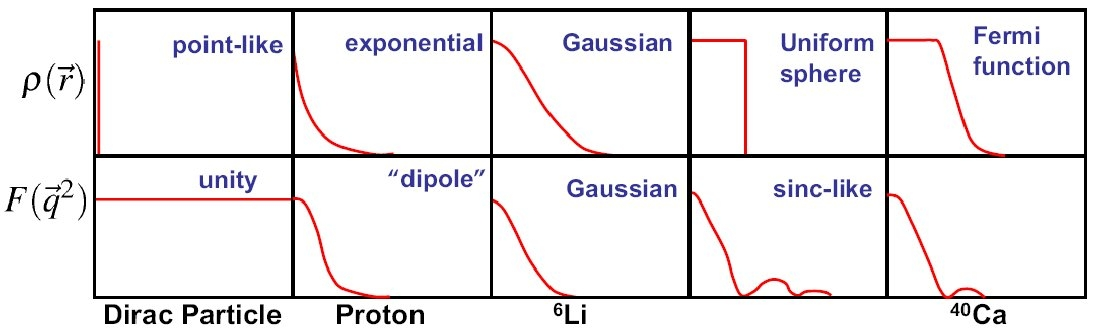
\includegraphics[width=\linewidth]{rho_vs_FF}
    \caption{Characristic of FF w.r.t. different density distribution functions}
\end{figure}

At small $\vec{q}^2$ limitation, one can do the Fourier expansion:
\begin{equation*}
    \begin{aligned}
	F(q^2) &= 4\pi \int r \rho(r) \frac{\sin{(qr)}}{q} dr \\
	    &= 4\pi \int \rho(r) r \left( r - \frac{1}{6} q^2r^3 + \cdots \right) dr	\\
	    &= \int \rho(r)  \left( 1 - \frac{1}{6} q^2r^2 + \cdots \right) 4\pi r^2 dr	\\
	    &= 1 - \frac{1}{6}q^2\langle r^2 \rangle + \cdots \\
	    &= F(0) + \left.\frac{dF}{dq^2}\right|_{q^2=0} \times q^2 + \cdots	\\
    \end{aligned}
\end{equation*}

and easily to get:
\begin{equation}
    \langle R^2 \rangle = -6 \left. \frac{dF(q^2)}{dq^2} \right|_{q^2 = 0}
\end{equation}
This equations prompts how to measure RMS radius:
one can measure the FF at some low $q^2$ points, extrapolate them 
to $q^2 = 0$, then the slope at $q^2 = 0$ will be the RMS radius (that's why
we use the RMS radius rather than the more physical definition of: 
$\langle R \rangle = \int d^3\vec{r} \ r \ \rho(\vec{r})$).

For charged proton, the FF will be the precisely measured EM FF:
\begin{equation}
    \langle R_p^2 \rangle = -6 \left. \frac{dF_{EM}(q^2)}{dq^2} \right|_{q^2 = 0}
\end{equation}
While neutron is neutral, we will measure its RMS radius from its weak charge
distribution:
\begin{equation}
    \langle R_n^2 \rangle = -6 \left. \frac{dF_{weak}(q^2)}{dq^2} \right|_{q^2 = 0}
\end{equation}

The difference between them will be what we called the neutron skin thickness
\begin{equation}
    R_{skin} = R_n - R_p 
\end{equation}

The neutron skin, as its name implies, is founded in neutron-rich isotopes that
have more neutrons than protons. An intuitive picture is following: analog to
atomic electron shell model, protons and neutrons also arrange themselves on
shelles from low to high energy, without disturbing each other (nuclear shell model).
The higher the energy level, the larger the orbit (radius).
For most nuclei, they have similar number of proton and neutron, therefore an 
approximative proton and neutron radius. But for neutron-rich isotopes, the extra neutrons
need to stay on higher energy shell after filling all low energy ones, forming
a larger radius than proton and therefore the neutron skin.

Of course, this picture is too simple to fully understand the neutron skin.
One quick question will be how can one ensure that the extra neutrons lies 
in the surface rather than the core area? That's related to the symmetry energy, 
more specifically, the density dependence of the symmtery energy. 
Because the core area has a 
higher nucleon density than the surface, and symmetry energy represents the 
penalty for breaking the proton-neutron symmetry: the higher the density, the
larger the symmetry energy, therefore the lower the binding energy (the energy
needed to break down a nuclear system: $BE(N, Z) = M(N, Z)c^2 - Zm_p c^2 - Nm_n c^2$), the less
stable the nuclei. So it is symmetry energy that pushes extra neutrons to 
the surface, which is the deeper reason for the formation of neutron skin.
% the more nucleons on surface, the stronger the surface tension, therefore
% surface tension favorsl leaving extra neutrons in the core area

Experimental hints of the existance of the neutron skin comes from optical isotope
shifts (FIXME)
%%%%%%%%%%%%%%%%%%%%%%%%%%%%%%%%%%%%%%%%%%%%%%%
\subsection{Theorectical Models} 
\label{subsec:models}
Though we don't know the actual neutron distribution, one would not expect too
much difference between the proton and neutron distributions, and we know the
proton distribution very well, through elastic ep scattering. 
The scattering cross section is:
\begin{equation}
    \frac{d\sigma}{d\Omega} = \left( \frac{d\sigma}{d\Omega} \right)_{Mott} |F(q^2)|^2
\end{equation}

FF encodes information about the charge structure of a nucleon, it is an interference
effect, finite size of the scattering center introduces a phase difference between
different plane waves scattered from different points in space.
\begin{figure}    
    \centering
    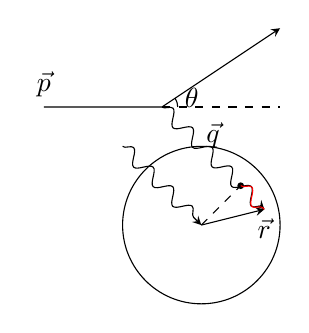
\begin{tikzpicture}
	\draw (0, 0) circle (1 cm);
	\draw[fill=black] (0.5, 0.5) circle (1 pt);
	\draw[-stealth] (-2, 1.5) node [above] {$\vec{p}$} -- ++(1.5, 0) -- ++(1.5, 1);
	\draw[-stealth, decorate, decoration=snake] (-1, 1) -- (0, 0);
	\draw[dashed] (-0.5, 1.5) -- +(1.5, 0);
	\draw (-0.3, 1.5) arc (0:34:0.2) node[right] {$\theta$};
	\draw[-stealth, decorate, decoration={snake}] (-0.5, 1.5) -- node[above] {$\vec{q}$} (0.8, 0.2);
	\draw[-stealth] (0, 0) -- (0.8, 0.2) node[below] {$\vec{r}$};
	\draw[dashed] (0, 0) -- (0.5, 0.5);
	\draw[red, decorate, decoration=snake] (0.5, 0.5) -- (0.8, 0.2) ;
    \end{tikzpicture}
    \caption{As we can see, the virtual photon wave absorbed by a nucleon at position
    $\vec{r}$ will travel a further distance $\vec{q}\cdot\vec{r}$ than the one
    absorbed at the central point, therefore a phase difference $e^{i\vec{q}\vec{r}/\hbar}$}
    \label{fig:FF_phase_diff}
\end{figure}

Consider the simplest hard ball model:
\begin{equation*}
    \rho(r) = 
    \begin{cases}
	\frac{3}{4\pi R^3}  & r \le R	\\
	0		    & r > R   \\
    \end{cases}
    \label{eqn:hard_ball_model}
\end{equation*}
Then the FF will be:
\begin{equation*}
    F(q^2) = \frac{3}{(qR)^3} \left( \sin(qR) - qR\cos(qR) \right)
\end{equation*}
where $q = 2p\sin(\theta/2)$

Given the Mott cross section:
\begin{equation}
    \left( \frac{d\sigma}{d\Omega} \right)_{Mott} = 
    \begin{cases}
	\frac{Z^2 \alpha^2}{4E^2\sin^4(\theta/2)}\cos^2(\theta/2)   
	    & \text{light nuclei} \ Z\alpha << 1  \\
	\frac{Z^2 \alpha^2}{4E^2\sin^4(\theta/2)}\cos^2(\theta/2) \left[ 1 + \pi Z \alpha \frac{\sin(\theta/2)(1-\sin(\theta/2)))}{\cos^2(\theta/2)}\right]   
	    & \text{medium nuclei}  \\
    \end{cases}
\end{equation}
We can draw the cross section, as a function of scattering angle in Fig. \ref{fig:ca_xsec}.
\begin{figure}
    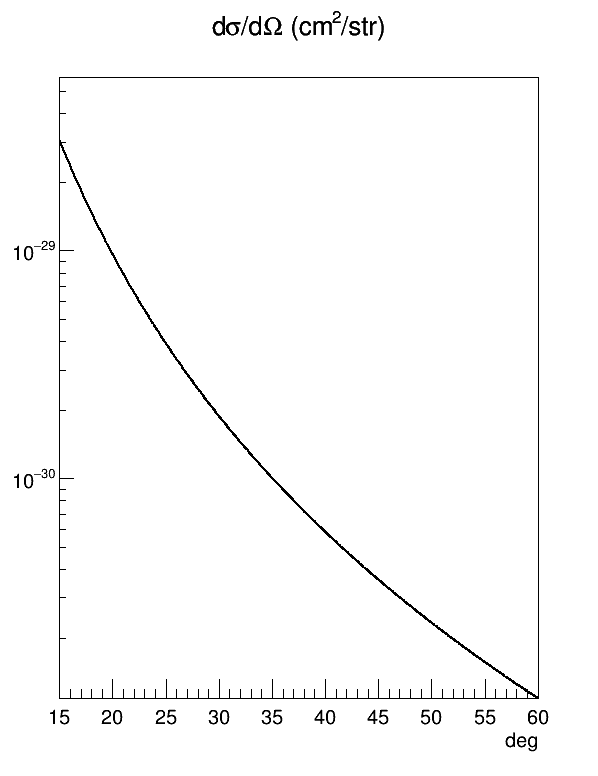
\includegraphics[width=0.32\linewidth]{ca48_xsec_mott}
    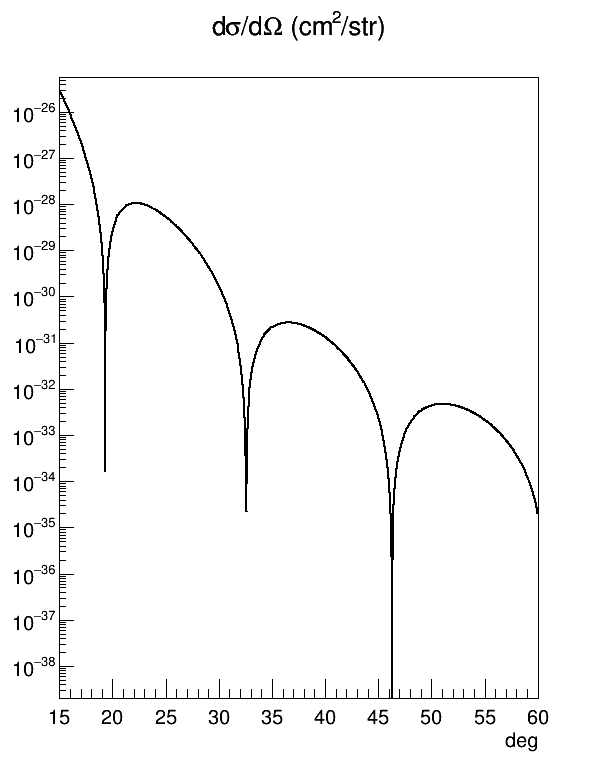
\includegraphics[width=0.32\linewidth]{ca48_xsec_hard_ball}
    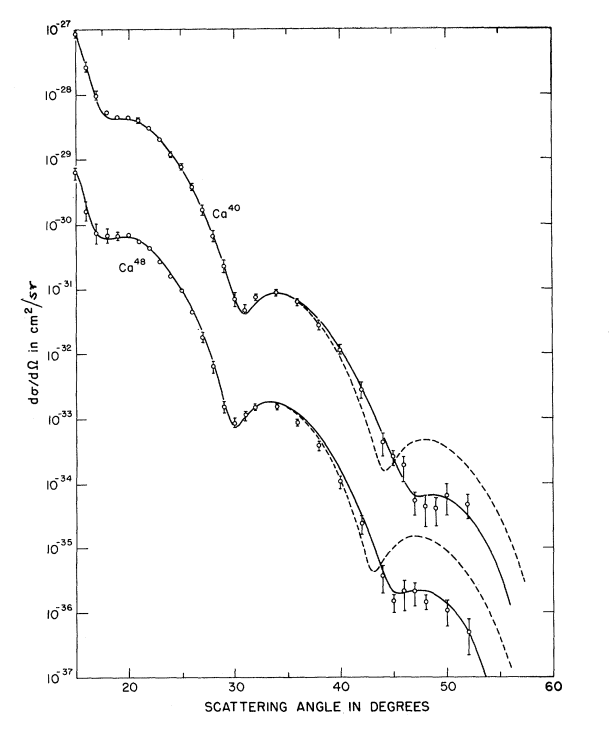
\includegraphics[width=0.32\linewidth]{ca_xsec_exp}
    \caption{Left: Mott cross section of electron elasticaly scattered off a Ca48
    target. Parameters: $p=E=757.5 \ MeV$.
    Middle: cross section of electron elasticly scattered off Ca48 with the hard ball
    model (\ref{eqn:hard_ball_model}). Parameters: $E =  757.5\ MeV$, $R=A^{1/3}\ fm$. 
    Right: experimental values (dots) and theoretical prediction (solid line),
    their calculation assumed the charge distribution as a Fermi 3-parameter function.
    $\rho(r) = \frac{\rho_0(1 + \omega r^2/c^2)}{1 + exp((r-c)/a)}$. The \Ca \ (\ca)
    cross sections are multiplied by $10^{-1}$ ($10$) to seperate them.  
    \cite{PhysRevLett.19.527}
    }
    \label{fig:ca_xsec}
\end{figure}

Well, the hard ball model doesn't reproduce the experimental distribution, it does
characterize the real distribution and show us how FF modify the Mott cross section:
the oscillating dips. As it turns out, a more realistic model will be the
Saxon-Woods distribution (also called the Fermi 2-parameter model or the Fermi
distribution):
\begin{equation}
    \rho(r) = \frac{\rho(0)}{1 + exp((r-R)/t)}
\end{equation}
where $R = (1.2A^{1/3} - 0.48) \ fm$ denotes the nuclear force radius, 
and $t = 0.4-0.5 \ fm$ for  $A > 40$.
\begin{figure}
    \centering
    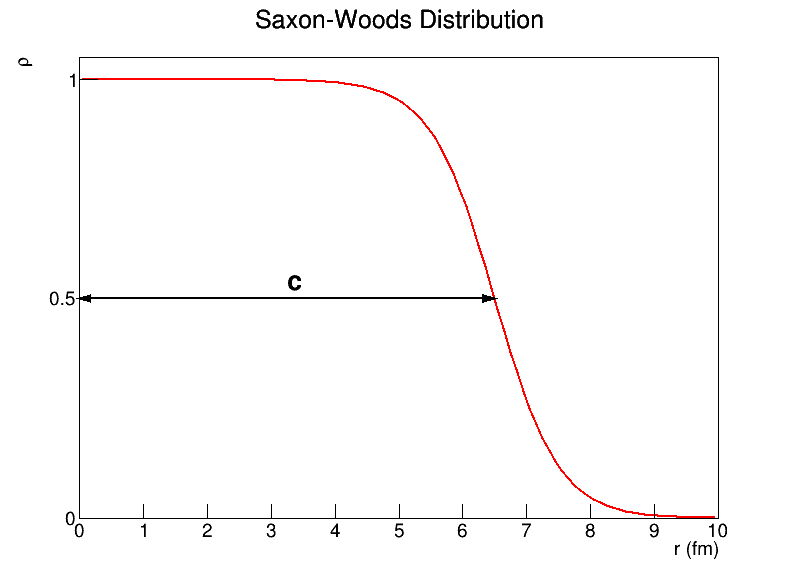
\includegraphics[width=0.5\linewidth]{fermi_distribution}
    \caption{In nuclear Shell Model, it is assumed that nucleons occupy 
    different eigenstates of the same spherically symmetric average potential.
    This potential, unlike that in atomic shell model, needed to be guessed. 
    It turns out that the Saxon-Woods model is a good candidate: 
    $V(r) = -\frac{V(0)}{1+exp((r-c)/a)}$ (c is the half-height raidus and a represents
    diffuseness of the distribution). Because the potential is formed
    by all nucleons, so it is approximatively proportional to the nucleon density, 
    therefore the same distribution for nucleon density.} 
\end{figure}
The right plot on Fig. \ref{fig:ca_xsec} uses a fine tuned Fermi 3-parameter model,
which fits quite well with the data. More detailed discussion about the Fermi 
distribution can be found in \cite{Maximon:1966sqn}.
% \begin{equation}
%     \rho(r) = \frac{\rho_0(1 + \omega r^2/c^2)}{1 + exp((r-c)/a)}
% \end{equation}

One theoretical model based on the Fermi distribution is the FSUGold \cite{PhysRevLett.95.122501},
the neutron distribution of \Pb predicted by FSUGold is shown in Fig. \ref{fig:FSUGold_pb208}.
\begin{figure}[h!]
    \centering
    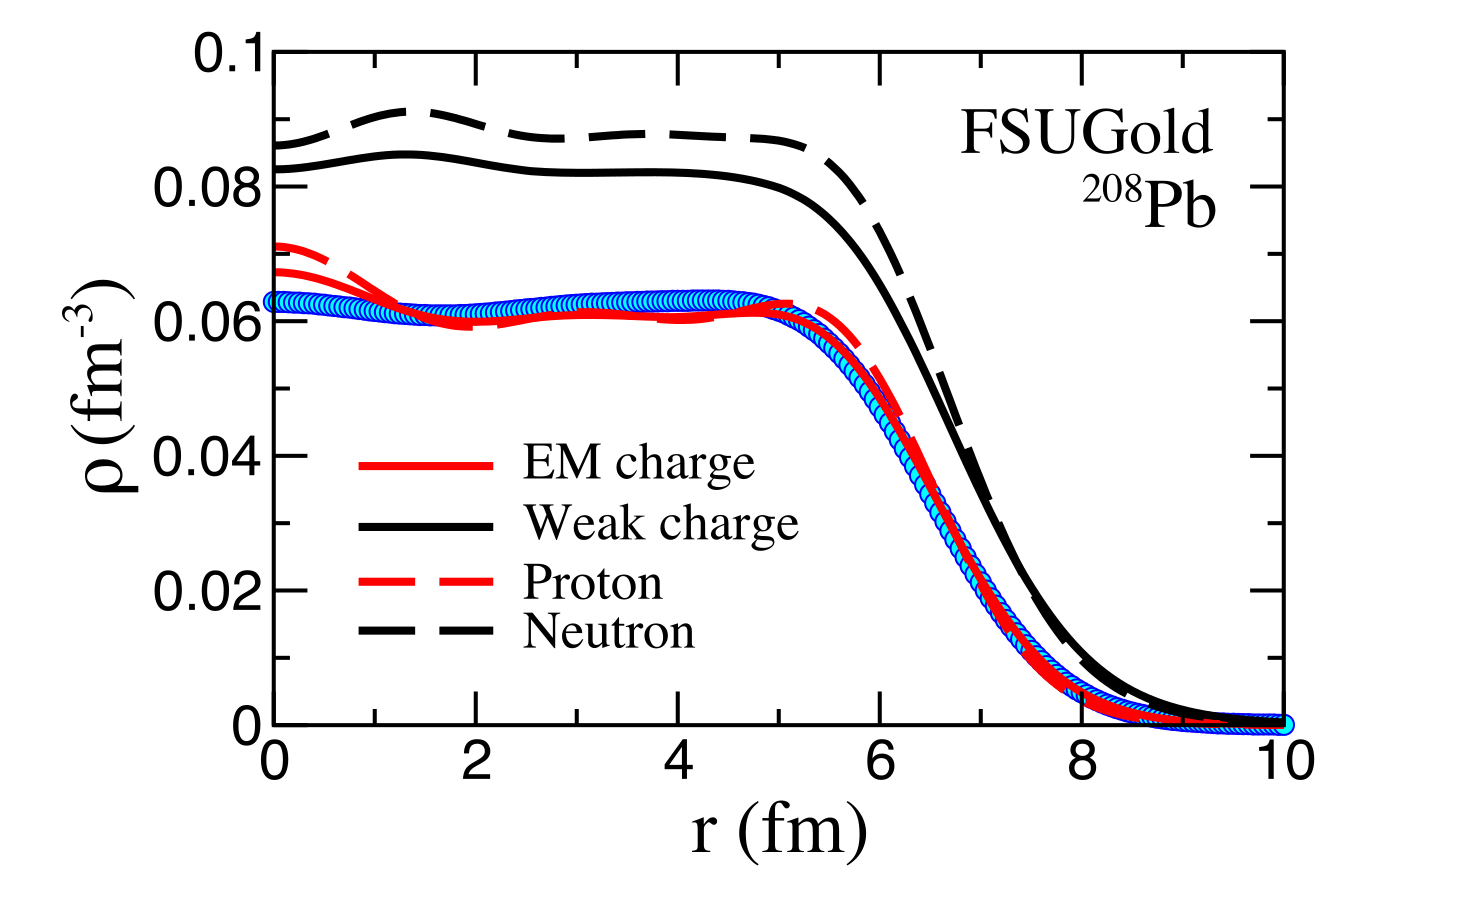
\includegraphics[width=0.6\linewidth]{FSUGold_pb208}
\end{figure}

We also need to note that for medium and heavy nuclei, the Born approximation
doesn't hold, where the incoming and outgoing waves are treated as plane waves.
In reality, the waves are distorted by the intense nuclear EM field, making them
no longer plane waves any more. So we have to take into account the 
Coulomb distortion effect, which will modify the PV asymmetry significantly.
Coulomb distortion can be understood as multiple EM interactions with
the same nucleus, so the distortion correction is proportional to $Z\alpha$. 
Obviously, this correction is more important for \Pb because of its large Z value,
Coulomd-distortion could reduce the PV asymmetry by as much as 30\% as we can see
in the following plots.


With these information, one is able to solve the Dirac equation directly to know
the PV asymmetry, as shown in the following 2 plots:
\begin{figure}[h!]
    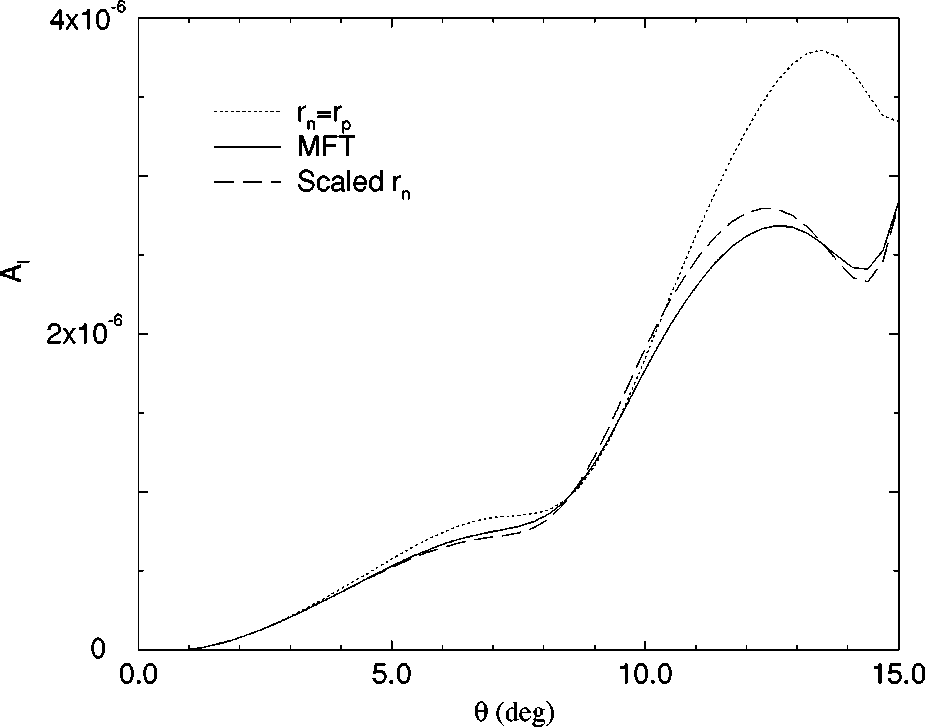
\includegraphics[width=0.49\linewidth]{Coulomb_distortion_Pb208}
    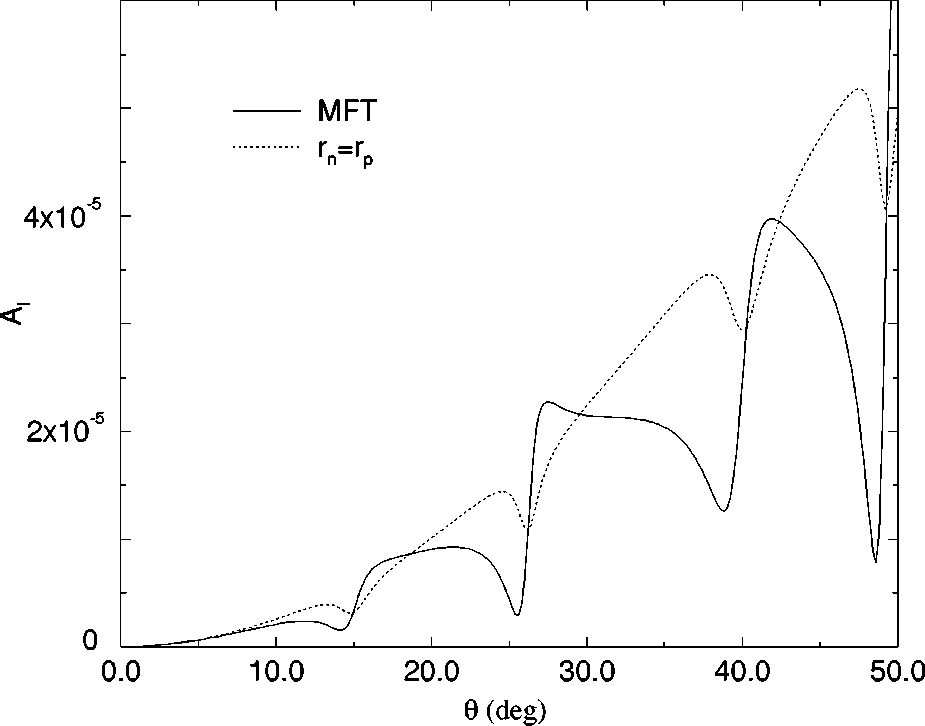
\includegraphics[width=0.49\linewidth]{Coulomb_distortion_Ca48}
    \caption{PV asymmetry for \Pb and \Ca versus scattering angle at 850 MeV 
    (Coulomb distortion correction included). 
    The dotted curve assumes the same weak and charge distribution, 
    while the solid curve is based on relativistic Mean Field Densities. The
    dashed curve in \Pb plot uses 3 parameter Fermi distribition \cite{PhysRevC.57.3430}}
\end{figure}


% 1. neutron distribution
% 2. symmetry energy dependence on density
%%%%%%%%%%%%%%%%%%%%%%%%%%%%%%%%%%%%%%%%%%%%%%%%%%%%%%%%%%%%%%%%%%%%%%%%
\section{Symmetry Energy} 
% what's symmetry energy
% why it is important
% how to know/measure it -- theoritically and experimentally
% the energy difference between a pure neutron star and a corresponding symmetric
% nuclear matter
It has long been a hot topic for nuclear scientists to study how the asymmetry 
between number of proton and nucleon will affect nuclei, especially the binding
energy, which hints us the limit of new isotope elements. Using the simplest 
Liquid Drop Model (LDM), we will get the Bethe-Weizsacker Semi-empirical Mass Foumula:
\begin{equation}
    \label{eq:mass-foumula}
    \begin{gathered}
	E\ (MeV) = \textcolor{black}{a_V A} 
	    - \textcolor{blue}{a_S A^{2/3}} 
	    - \textcolor{green}{a_C\frac{Z(Z-1)}{A^{1/3}}} 
	    - \textcolor{red}{a_A\frac{(N-Z)^2}{A}} 
	    + \textcolor{cyan}{\delta(A, Z)} \\
	\delta(A, Z) = 
	    \begin{cases}
		+\delta_0	& \text{Z, N even} \\
		0		& \text{A odd}	\\
		-\delta_0	& \text{Z, N odd (A even)} \\
	    \end{cases}
    \end{gathered}
\end{equation}

\begin{itemize}
    \color{black} \item Volume term: nucleons attract nearest neighbors 
	through strong force ($a_V \sim 16\ MeV$), reflects the short-range
	nature of strong interaction.
    \color{blue}  \item Surface term: correction to the volume term -- nucleons 
	on the surface aren't completely surrounded by other nucleons
    \color{green} \item Coulomb term: EM charge repulsion
    \color{red}   \item Asymmetry term: Pauli exclusion principle
    \color{cyan}  \item Pairing term: spin coupling effect -- if N and Z are even,
	then the nuclei will be stable thanks to the occurance of 'paired spin';
	on the other hand, nuclei with odd number of proton and neutron are usually
	unstable. ($\delta_0 \sim 1\ MeV$, slowly decreasing with A)
\end{itemize}

The first 3 terms are natural and easy to understand, while the 4th term is 
not so obvious. It is based only on Pauli exclusion principle. In heavy nuclei,
more neutrons than protons are needed to balance the repulsion between protons.
Due to the Pauli exclusion principle, these extra neutrons' energy will be 
higher than the rest of nucleons, therefore introducing this correction term.

Regard the nuclear system as a free Fermi gas of protons and neutrons, then the 
kinematic energy of this system will be:
$$ E_k = E_N + E_Z = \frac{3}{5}ZE_F^p + \frac{3}{5}NE_F^n $$
Since the Fermi energy is proportional to $n^{2/3}$
$$ E_k = C(Z^{5/3} + N^{5/3})  $$
Expanse it in terms of N-Z \ref{ap:symmetry_energy}, we will get
\begin{equation*}
    \begin{aligned}
	E_k &= 2^{-2/3}C\left(A^{5/3} + \frac{5}{9}\frac{(N-Z)^2}{A^{1/3}} \right) + O((N-Z)^4) \\
	    &= \frac{3}{5} E_F A + \frac{1}{3}E_F\frac{(N-Z)^2}{A} + O((N-Z)^4) \\
    \end{aligned}
\end{equation*}
The first term contributes to the volume term and the second term is minus the 
asymmetry term because $E_k$ contributes to the binding energy negatively.

For a general discussion, we can ignore the 3rd term to focus on the homogeneous
nuclear (residual strong) interaction between nucleons, and the 5th term which is too small.
Now, we can talk about any nuclear system composed of Z protons (EM charge-less) 
and N neutrons, rather than just true nuclei. Now we have a simplified equation
of state (EoS) for nuclear matter:
\begin{equation}
    \label{eq:modified-mass-formula-1}
    \begin{aligned}
	E &= a_V A - a_S A^{2/3} - a_A\frac{(N-Z)^2}{A}  \\
	e &= \frac{E}{A} = a_V - a_S A^{-1/3} - a_A\frac{(N-Z)^2}{A^2}
    \end{aligned}
\end{equation}

Actually, we should also discard the second term. Obviously, we can't guarantee
any specific shape about the nuclear system; what's mroe, for what people model
with most -- the infinite nuclear system, we don't need to consider the surface 
term at all.
\begin{equation}
    \label{eq:modified-mass-formula-2}
    \begin{aligned}
	E &= a_V A - a_A\frac{(N-Z)^2}{A}  \\
	e &= \frac{E}{A} = a_V - a_A\frac{(N-Z)^2}{A^2} = e_0(A) - a_A\beta^2 
    \end{aligned}
\end{equation}
Here we define $\beta = \frac{N-Z}{A}$ as asymmetry between the number of protons and neutrons. 

For infinite system, density, instead of A, will be a better choice to parameterize
the EoS. So we should replace N, Z and A with their corresponding density: $\rho_n$, 
$\rho_p$ and $\rho$ ($\beta = \frac{\rho_n - \rho_p}{\rho}$). 
So we are considering an infinite uniform nuclear system at 0 temperature that interacts
only via the nuclear force. For any identified $\rho$,
eq \eqref{eq:modified-mass-formula-2} will be:
\begin{equation}
    \label{eq:symmetry-energy}
    e(\rho, \beta) = e(\rho, 0) + S(\rho)\beta^2 + O(\beta^4)
\end{equation}

This is an expansion of the binding energy per nucleon around $\beta = 0$.
Due to the isospin symmetry between proton and neutron, any isoscalar quantities
F will keep unchanged under $n \leftrightarrow p$ interchange, while isovector 
% change all n into p and p into n. Not just one proton and one neutron
quantities G will change sign. $\beta$ is an isovector, so for a smooth $F(\beta)$,
its expansion around $\beta = 0$ has even terms only:
$$ F(\beta) = F_0 + F_2\beta^2 + F_4\beta^4 + \dots $$
On the other hand, for a smooth $G(\beta)$, its expansion around $\beta = 0$ has
odd terms only:
$$ G(\beta) = G_1\beta + G_3\beta^3 + \dots $$

e is an isoscalar, it doesn't change under $n \leftrightarrow p$ interchange 
as we can see from eq \eqref{eq:modified-mass-formula-2}. The coefficient 
$S(\rho) = \frac{\partial^2 e (\rho, \beta)}{\partial \beta^2}$ is
what we call the \textbf{symmetry energy}, a key parameter in explaining a wide
range of nuclear properties and phenomena. It describes how much energy will be
released when exchange all protons into neutrons for a symmetric nuclear system. 
% a plot for symmetry energy from some models

Not only is $S$ itself important, but also its dependence on $\rho$. 
By convention, $S(\rho)$ is expanded around the nuclear saturation density $\rho_0$
(following the free Fermi gas assumption):
\begin{equation}
    S(\rho) = S(\rho_0) 
    + \left.\frac{dS}{d\rho}\right|_{\rho_0}(\rho - \rho_0)
    + \frac{1}{2}\left.\frac{d^2S}{d\rho^2}\right|_{\rho_0}(\rho - \rho_0)^2
    + \frac{1}{6}\left.\frac{d^3S}{d\rho^3}\right|_{\rho_0}(\rho - \rho_0)^3
    + \dots
\end{equation}
From which, we have some auxiliary parameters defined:
\begin{equation}
    \begin{aligned}
	S_0 &= S(\rho_0)	\\
	L   &= 3\rho_0\left.\frac{dS}{d\rho}\right|_{\rho_0}	\\
	K_{sym}	&= 9\rho_0^2\left.\frac{d^2S}{d\rho^2}\right|_{\rho_0}	\\
	Q_{sym}	&= 27\rho_0^3\left.\frac{d^3S}{d\rho^3}\right|_{\rho_0}	\\
    \end{aligned}
\end{equation}
Among them, L represents S's dependence on $\rho$.

Take neutron star \cite{Lattimer.2001} as an example, it has most neutrons and 
a few protons, so its $\beta = 1$.
\begin{equation}
    \label{eq:neutron-star}
    \begin{aligned}
	 E = E_0 + S	\\
	 P = \rho^2 \frac{dS}{d\rho} \approx \frac{L\rho^2}{3\rho_0}	\\
	 RP^{-1/4} \approx const    \\
    \end{aligned}
\end{equation}
The amazing thing is that neutron star's pressure dependents on L is proportional
to $R^4$. Once we know the L value, we will know the pressure and therefore the 
radius of a neutron star. % (Do all neutron stars have the same $\rho$ and R ???)

Being such an important parameter, a great effort has been done to extract S 
and L. Comparing \eqref{eq:modified-mass-formula-2} and \eqref{eq:symmetry-energy},
we can directly get:
\begin{equation}
    S(\rho) \approx -a_A
% S(\rho) = -a_A + \frac{L}{3}\frac{\rho - \rho_0}{\rho_0}
\end{equation}
But this tells us only the symmetry energy at nuclear density ($1.22 \times 10^{44}\ m^{-3}$),
what about the symmetry energy at other density values? Especially at the nuclear
saturation density ($\sim 1.7 \times 10^{44}\ m^{-3}$)? And what about its density
dependence? Another strategy is the energy density functionals (EDF), which fits
the binding energy throughout the nuclear mass table to find out the best EDF,
then use it to calculate $S(\rho)$. Fitting parameterizations are constrained
by nuclear density, proton RMS radii and nuclear binding energies. 
The problem is many EDFs can fit equally well with these constrains, but have quite 
different L values, as shown in Fig. \ref{fig:neutron_EOS}.
If there is a experiment that can identify S (L) value without model dependence, 
then no doubt it will help a lot in understanding the symmetry energy and the EoS.
\begin{figure}
    \begin{subfigure}[c]{0.5\textwidth}
	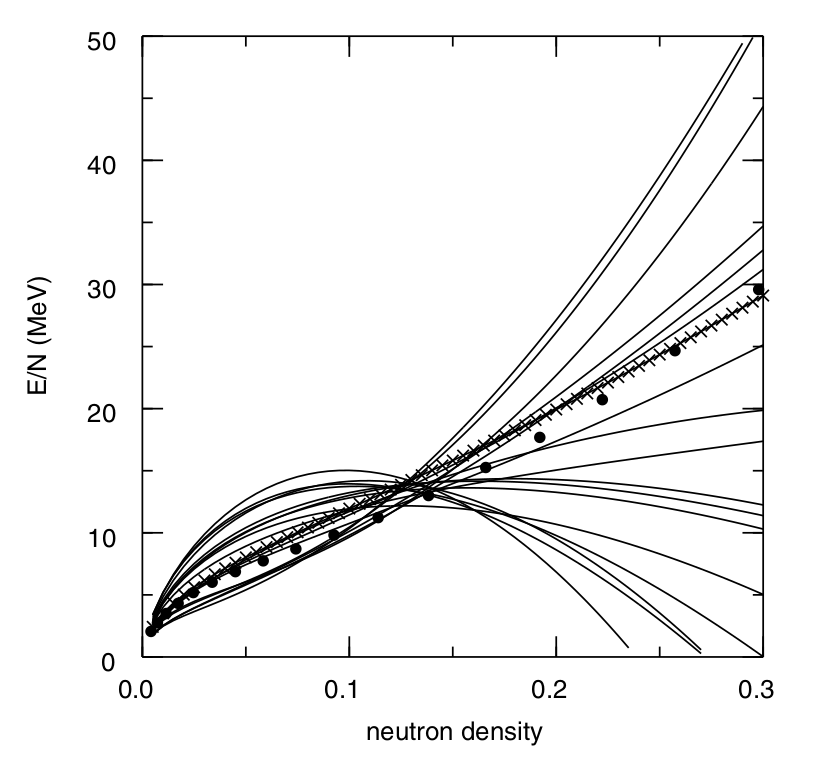
\includegraphics[width=\linewidth]{S_vs_rho_n}
	\caption{Neutron EOS for 18 Skyrme parameter sets. The filled circles are
	the Friedman-Panharipande (FG) variational calculations and the crosses are SkX. 
	\cite{PhysRevSTAB.7.042802}
	We can see different models have very different symmetry energies.
	}
    \end{subfigure}
    \begin{subfigure}[c]{0.5\textwidth}
	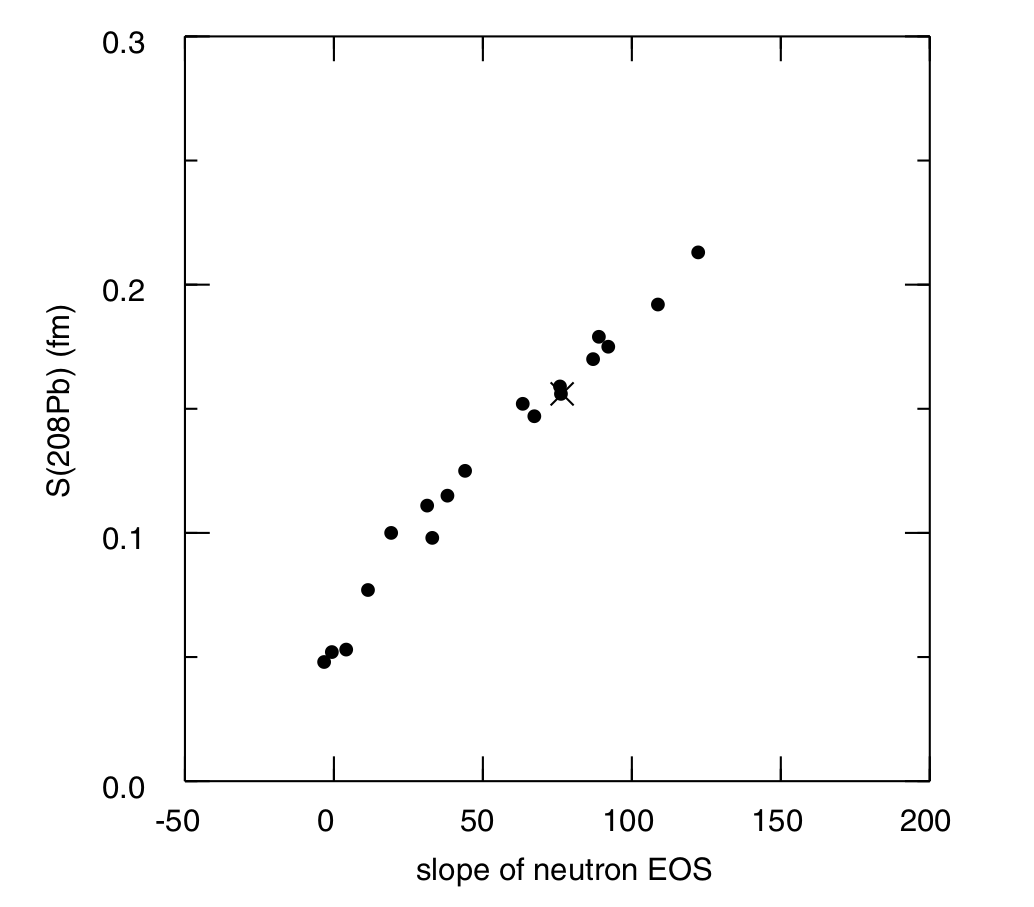
\includegraphics[width=\linewidth]{S_Pb_in_S_N_EOS}
	\caption{Symmetry energy for neutron EOS at $\rho_n = 0.1 \text{neutron}/fm^3$
	(in units of MeV $fm^3$/neutron) vs the S value in \Pb for 18 Skyrme parameter sets. 
	The cross is SkX. Determination of S in \Pb will greatly constrain the 
	possible candidates.}
    \end{subfigure}
\end{figure}
% experiments that measure L

% neutron skin
The method to measure L in lab is to measure the neutron skin thickness of 
neutron rich nuclei. For symmetric nuclei (N = Z), the protons and neutrons are
expected to distribute uniformly. While for neutron-rich nuclei, the extra 
neutrons are pushed out against the surface tension\cite{PRL.85.5296}, therefore
forming a neutron skin. 

Neutron skin and neutron star, though of their 18 orders of magnitude difference 
in size (fm vs km), both are neutron-rich nuclear matter and governed by the 
same physical laws: eq \eqref{eq:neutron-star}. So by measuring the neutron
skin thickness, we can derive P and L values, for the study of neutron stars
and nuclear EoS.

%%%%%%%%%%%%%%%%%%%%%%%%%%%%%%%%%%%%%%%%%%%%%%%%
\section{Physics Beyond the Standard Model (SM)} 
Parity-Violating Electron Scattering is always a promising avenue for physics
beyond the SM in precision frontier.
Flavor conserving interaction:
$$ |A_\gamma + A_Z + A_{new}|^2 \rightarrow A^2_\gamma\left[ 1 + 2\frac{A_Z}{A_\gamma}
 + 2\frac{A_{new}}{A_\gamma} \right]$$

%%%%%%%%%%%%%%%%%%%%%%%%%%%%%%%%%%%%%%%%%%%%%%%%
\section{Asymmetry}
\subsubsection{Parity}

\begin{figure}[h!]
    \centering
    \begin{tikzpicture}[decoration={markings, 
	mark=at position 0.5 with {\arrow{stealth}}}
	]
	\begin{scope}
	    \coordinate (O) at (0, 0);
	    \filldraw[black] (O) circle (1pt);
	    \node[red, above] at (O) {$G_F$};
	    \draw[postaction={decorate}] (-2, 0) node[above] {n} -- +(2, 0);
	    \draw[postaction={decorate}] (O) -- +(2, 0)node[above] {$p$} ;
	    \draw[postaction={decorate}] (O) -- (35:2) node[above, sloped] {$e^-$};
	    \draw[postaction={decorate}] (O) -- (-35:2) node[above, sloped] {$\bar{\nu}_e$};
	\end{scope}

	\begin{scope}[xshift=5cm]
	    \coordinate (O) at (0, 0);
	    \filldraw[black] (O) circle (1pt);
	    \node[red, above] at (O) {$G_F$};
	    \draw[postaction={decorate}] (-2, 0) node[above] {n} -- +(2, 0);
	    \draw[postaction={decorate}] (O) -- +(2, 0)node[above] {$p$} ;
	    \draw[postaction={decorate}] (O) -- (35:2) node[above, sloped] {$e^-$};
	    \draw[postaction={decorate}] (-35:2) node[above, sloped] {$\nu_e$} -- (O);
	\end{scope}
    \end{tikzpicture}
    \caption{Fermi's interpretation of beta decay, current $j_{n \rightarrow p}$ 
    convert n into p and current $j_{\nu_e \rightarrow e}$ creates $(e, \ \bar{\nu}_e) $
    pair.}
\end{figure}
The story traces back to the early age of particle physics. To explain the beta decay, 
Fermi proposed the 4-fermion interaction 
(Fermi's interaction) in 1933 \cite{Fermi1934}, which is a low-energy limit of the 
weak interaction. In his theory, In analogy to the EM interaction (emission of a
photon by an electron: $\CM = ej_\mu^{em} A^\mu$) Fermi interpretted the $\beta$
decay as emission of a $(e, \bar{\nu}_e)$ pair, during the process neutron converts
itself into a proton, therefore coupling of two current:
\begin{equation}
    \CM = G_F (\bar{p} \mathds{O}^\mu n)(\bar{e} \mathds{O}_\mu \nu_e) 
	= G_F j^\mu_{(n\rightarrow p)} j_\mu^{(\nu_e\rightarrow e)}
\end{equation}
Where $G_F = 1.166 \times 10^{-5} \ (GeV)^{-2}$ is the coupling constant that 
will be experimentally determined and $\mathds{O}$ represents 
the possible operators. Out of the 5 possible Lorentz invariant bilinear forms 
(Scalar (S: $\mathds{O} = \mathds{1}$), pseudoscalar (P: $\mathds{O} = \gamma^5$), 
Vector (V: $\mathds{O} = \mathds{\gamma^\mu}$), Axial vecotr (A: $\mathds{O} = \gamma^\mu\gamma^5$) 
and Tensor (T: $\mathds{O}=\sigma^{\mu\nu} = \frac{i}{2}(\gamma^\mu\gamma^\nu - \gamma^\nu\gamma^\mu)$)),
Fermi selected the vector current to keep in line with the EM interaction:
$j^\mu = \bar{u} \gamma^\mu u$.

In 1956, T. D. Lee and C. N. Yang, both being Fermi's student, postulated the
revolutionary idea of parity violation for solving the $\tau-\theta$ puzzle, 
and they succeeded. Only one year later, their hypothesis was experimentally tested
by Wu etc in the decay of polarized $Co^{60}$ nuclei, establishing the fact
that parity is not conserved in weak interaction and therefore the weak 
current is not a pure vector-like quantity. 
Based on the experimental fact that parity is maximally violated \cite{PhysRev.109.1015}, 
Sudarshan and Marshak \cite{PhysRev.109.1860.2}, 
also Feymann and Gell-Mann \cite{PhysRev.109.193}
updated Fermi's theory by replacing the vector current with a new current to 
accomodate parity violation, which led us to:
\begin{equation}
    \CM = \frac{G_F}{\sqrt{2}}(\bar{p} \gamma^\mu(\mathds{1} - \gamma^5) n) (\bar{e} \gamma_\mu(\mathds{1} - \gamma^5) \nu_e)
\end{equation}
The factor of $\frac{1}{\sqrt{2}}$ was introduced to keep $G_F$ unchanged (Fermi's
original theory was not aware the fact that neutrino was left-handed only, resulting
in a decay phase space twice the real value in nature, to fix the problem, we can
either modify the value of $G_F$ or introduce a correction factor $\frac{1}{\sqrt{2}}$).
The V and A parts of V-A theory refer to the vector and axial vector current, 
responsible for Fermi transitions and Gamow-Teller transitions respectively.
\begin{equation}
    j_V^\mu = \bar{u}\gamma^\mu u   \qquad 
    j_A^\mu = \bar{u}\gamma^\mu\gamma^5 u   
\end{equation}
The form of V-A as $\mathds{1} - \gamma^5$ happens to be the projection operator:
\begin{equation}
    P_R = \frac{\mathds{1} + \gamma^5}{2}   \qquad P_L = \frac{\mathds{1} - \gamma^5}{2}
\end{equation}
By definition of gamma matrix, one can easily verify that:
\begin{equation}
    \begin{gathered}
	\left(\frac{\mathds{1} - \gamma^5}{2} \right)^2 = \frac{\mathds{1} - \gamma^5}{2} 
	\qquad 
	\gamma^\mu \frac{\mathds{1} - \gamma^5}{2} = \frac{\mathds{1} + \gamma^5}{2} \gamma^\mu \\
	\gamma^\mu \frac{\mathds{1} - \gamma^5}{2} = \frac{\mathds{1} + \gamma^5}{2} \gamma^\mu \frac{\mathds{1}-\gamma^5}{2}
    \end{gathered}
\end{equation}
Then one can see the handness of the new current:
\begin{equation}
    \CM = \frac{4G_F}{\sqrt{2}}(\bar{p} \gamma^\mu\frac{\mathds{1} - \gamma^5}{2} n) (\bar{e} \gamma_\mu\frac{\mathds{1} - \gamma^5}{2} \nu_e) 
    = \frac{4G_F}{\sqrt{2}}(\bar{p}_L \gamma^\mu n_L)(\bar{e}_L \gamma_\mu \nu_{e,L})
\end{equation}
Only left (right)-handed particle (antiparticle) can interact in weak interaction.
In analogy to EM interaction, the coupling constant is proportional to a weak
charge (weak isospin $T_3$), then right-handed fermions (left-handed antifermions) 
will have $T_3 = 0$ and left-handed fermions have the same weak charge. 

Given the fact that the charge current (it changes particle's electric charge) 
connects 2 types of fermions and lepton number is conserved in weak interaction, 
it is natural to group them in a lepton doublet: $f_L = \begin{pmatrix} \nu_l \\ l \end{pmatrix}_L$.
This implies us that for left-handed fermions: $T=\frac{1}{2}, T_3 = \pm\frac{1}{2}$ 

Applying the V-A theory to more decay and scattering process (
$\mu^+ \rightarrow e^+ + \nu_e + \bar{\nu}_\mu$, $\pi^- \rightarrow l + \bar{\nu}_l$ etc.), 
we have 2 charge currents:
\begin{equation}
    j_\mu^- = \bar{\nu}_{e, L} \gamma_\mu e_L	\quad 
    j_\mu^+ = \bar{e}_L \gamma_\mu \nu_{e,L}
\end{equation}
which can be written in a more compact way w.r.t. the lepton doublet:
\begin{equation}
    j_\mu^\pm = \bar{f}_L \gamma_\mu t^\pm f_L
\end{equation}
where,
\begin{equation}
    t^+  =
    \begin{pmatrix}
	0   & 1	\\
	0   & 0	\\
    \end{pmatrix}
    = \frac{1}{2}(\sigma^1 + i\sigma^2)
    \quad
    t^-  =
    \begin{pmatrix}
	0   & 0	\\
	1   & 0	\\
    \end{pmatrix}
    = \frac{1}{2}(\sigma^1 - i\sigma^2)
\end{equation}
We can see clearly the SU(2) symmetry by the $t^\pm$ expression, the raising ($t^+$)
and lowing matrices ($t^-$) are the combination of the first 2 Pauli matrices.
Then one should consider the third component:
\begin{equation}
    j_\mu^3 = \bar{f}_L \gamma_\mu \frac{1}{2}t^3 f_L = \frac{1}{2} (\bar{\nu}_{e, L} \gamma_\mu \nu_{e, L} - \bar{e}_{L} \gamma_\mu e_L)
\end{equation}
This is a neutral current. But what does this neutral current represents for?
The then only known neutral current is the EM current, but neutrino is neutral, how
could it have a EM neutral current? The neutral current kept as a mystery until
Glashow, Salam and Weinberg postulated the GSW model, which interpretes $j^3$ as
part of a more complete neutral current that includes $j^{em}$ -- the so called
$SU(2)_L \times U(1)$.

One problem with Fermi's theory is that the cross section ($\sigma \sim G_F^2 E^2$) 
will diverge at high energy, to which the solution was the introduction of
mediating mesons: $W^\pm$. Unlike photon that mediats EM interaction, W boson
is charged, and has a heavy mass implied from the short-range nature of the
weak interaction. The introduction of W fields just make the weak interaction
more similar to the EM interaction:
\begin{equation}
    \CL = g_W(J^+W^+ + J^-W^-)
\end{equation}
\begin{figure}[h!]
    \centering
    \begin{tikzpicture}[decoration={markings, 
	mark=at position 0.5 with {\arrow{stealth}}}
	]
	\begin{scope}
	    \coordinate (O) at (0, 0);
	    \filldraw[black] (O) circle (1pt);
	    \node[red, above left] at (O) {$\frac{G_F}{\sqrt{2}}$};
	    \draw[postaction={decorate}] (-2, 0) node[above] {n} -- +(2, 0);
	    \draw[postaction={decorate}] (O) -- +(2, 0)node[above] {$p$} ;
	    \draw[postaction={decorate}] (O) -- (35:2) node[above, sloped] {$e^-$};
	    \draw[postaction={decorate}] (-35:2) node[above, sloped] {$\nu_e$} -- (O);
	\end{scope}

	\begin{scope}[xshift=5cm]
	    \coordinate (O) at (0, 0);
	    \coordinate (P) at (-35:2);
	    \filldraw[black] (O) circle (1pt);
	    \filldraw[black] (P) circle (1pt);
	    \node[red, above left] at (O) {$V_{ud}g_W$};
	    \draw[postaction={decorate}] (-2, 0) node[above] {n} -- +(2, 0);
	    \draw[postaction={decorate}] (O) -- +(2, 0)node[above] {$p$} ;
	    \draw[decorate, decoration=snake] (O) -- node[red, midway, below left] {$\frac{1}{M^2_W}$} (P);
	    \draw[postaction={decorate}] (P) -- +(20:1) node[above, sloped] {$e^-$};
	    \draw[postaction={decorate}] ($(P) + (-20:1)$) node[below, sloped] {$\nu_e$} -- (P);
	    \node[red, below] at (P) {$g_W$};
	\end{scope}
    \end{tikzpicture}
    \caption{W-boson exchange picture of $\beta$ decay}
\end{figure}

Given the similarity between weak interaction and EM interaction, it is natural
to unify them into a multiplet of gauge fields. Based on Yang and Mills' non-abelian 
guuge theory, Salam and Weinberg successfully came up with a unified 
framework for both interactions -- the $SU(2)_L \times U(1)$ structure firstly suggested 
by Glashow. The SU(2) part is generated by `weak isospin', the subscript L refers
to the fact that only left-handed fermions couple to gauge boson of SU(2), and the U(1)
part comes from the `weak hypercharge'. There are 4 vector bosons:
$$ W^1, W^2, W^3, B $$
These bosons will couple to both left-handed and right-handed fermions. For simplicity,
let's consider only the first generation leptons here:
\begin{equation}
    \psi_1 = \begin{pmatrix} \nu_e \\ e^-  \end{pmatrix}	\quad
    \psi_2 = \nu_{e,R}	\quad
    \psi_3 = e^-_R    \quad
\end{equation}

For the left-handed doublet $\psi_1$, it interacts to all bosons, 
so the covariant derivative is:
\begin{equation}
    D_\mu = \partial_\mu - ig\frac{\sigma^a}{2}W_\mu^a - ig'y_1B_\mu
\end{equation}
where $y_1$ is the hypercharge of $\psi_1$.
The corresponding coupling Lagrangian is:
\begin{equation}
    \CL_{int, L} = -i\bar{\psi}_1 \gamma^\mu (g\frac{\sigma^a}{2}W^a_\mu + g'y_1B_\mu) \psi_1
	= -i(g\vec{j}^\mu\vec{W}_\mu + g'y_1\bar{\psi}_1\gamma^\mu\psi_1 B_\mu)
\end{equation}
For right-handed singlests, they don't couple to weak vector bosons, 
therefore the covariant derivative for right-handed fermions is:
\begin{equation}
    D_\mu = \partial_\mu - ig'y_{2(3)}B_\mu
\end{equation}
$y_{2(3)}$ are the hypercharge of $\psi_{2(3)}$
and the Lagrangian:
\begin{equation}
    \CL_{int, R} = -ig'(y_2\bar{\psi}_2 \gamma^\mu \psi_2 + y_3\bar{\psi}_3\gamma^\mu \psi_3) B_\mu
\end{equation}
So the complete interacting Lagrangian is:
\begin{equation}
    \CL_{int} = \CL_{int, L} + \CL_{int, R} = -i(g\vec{j}^\mu \vec{W}_\mu + g'j^\mu_{Y} B_\mu)
    \label{eqn:GSW}
\end{equation}
where $\vec{j}^\mu$ is the weak isospin current, it couples to a weak 
isotriplet of vector bosons: $\vec{W} = (W^1, W^2, W^3)$ with
coupling strength $g$; and the weak hypercharge current 
$j^\mu_{Y} = \sum_{i=1}^3 y_i\bar{\psi}_i\gamma^\mu\psi_i$ couples to 
an isosinglet vector boson: $B^\mu$ with strength $g'$. 

Because the GSW model preserve the SU(2) structure we talked about before, 
therefore it is obvious to reproduce the charged current:
\begin{equation}
    W^\pm = \frac{1}{\sqrt{2}}(W^1 \mp iW^2)	\quad
    j^\pm = j^1 \pm ij^2
\end{equation}
\begin{equation}
    j^1W^1 + j^2W^2 = \frac{1}{\sqrt{2}}(j^+W^+ + j^-W^-)
\end{equation}

As for the other 2 bosons, there is no way to satisfy $y_1 = y_2 = y_3$ and 
$g'y_i = eQ_i$ at the same time, so B is not pure A. 
Since both fields are neutral, one can try to mix them, 
and get some result matching experimental results:
\begin{equation}
    \begin{pmatrix}
	A   \\
	Z   \\
    \end{pmatrix}
    =
    \begin{pmatrix}
	\cos\theta_W	& \sin\theta_W	\\
	-\sin\theta_W	& \cos\theta_W	\\
    \end{pmatrix}
    \begin{pmatrix}
	B   \\
	W^3 \\
    \end{pmatrix} 
    \Leftrightarrow
    \begin{pmatrix}
	B   \\
	W^3 \\
    \end{pmatrix}
    =
    \begin{pmatrix}
	\cos\theta_W	& -\sin\theta_W	\\
	\sin\theta_W	& \cos\theta_W	\\
    \end{pmatrix}
    \begin{pmatrix}
	A   \\
	Z	\\
    \end{pmatrix} \\
\end{equation}
The mixing angle is known as the Weinberg angle. 

Rewrite eq. \ref{eqn:GSW} in terms of $W^\pm$, $Z$ and $A$:
\begin{equation}
    \begin{aligned}
	i\CL = &\frac{g}{\sqrt{2}}(j^+W^+ + j^-W^-)	\\
	    &+ \sum_{i=1}^3\bar{\psi}_i\gamma^\mu \left\{ 
		\left[g\frac{\sigma^3}{2}\sin\theta_W + g'y_i\cos\theta_W\right] A_\mu
		+ \left[ g\frac{\sigma^3}{2}\cos\theta_W - g'y_i\sin\theta_W \right] Z_\mu 
	    \right\} \psi_i
    \end{aligned}
\end{equation}
where $g_W = g/\sqrt{2}$ is the coupling constant of weak charged current.

The neutral part can be expressed in corresponding charge:
\begin{equation}
    \begin{aligned}
	i\CL_{NC} &= \sum_{i=1}^{3} \bar{\psi}_i\gamma^\mu\psi_i
	\left[ 
	    \left(g\sin\theta_W I_3 + g'\cos\theta_W Y \right) A_\mu 
	    + \left(g\cos\theta_W I_3 - g'\sin\theta_W Y \right) Z_\mu 
	\right]	\\
	&= ej^\mu_{EM}QA_\mu + g_Zj^\mu_Z Q_Z Z_\mu \\
    \end{aligned}
\end{equation}
Where $I_3$ is the weak isospin and $Y$ is the weak hypercharge; Similarly, $Q$ is
the EM charge in unit of electron charge and $Q_Z$ is the weak neutral charge.
$e$ and $g_Z$ are coupling constant for EM and neutral weak interaction respectively.
With $I_3$ and $Y$ vary for different fermions, we have the following relationship:
% \begin{equation}
%     \begin{aligned}
% 	ej^{EM} &= g\sin\theta_Wj^3 + g'\cos\theta_Wj^Y	\\	
% 	g_Zj^{Z} &= g\cos\theta_W j^3 - g'\sin\theta_W j^Y	\\
%     \end{aligned}
% \end{equation}
\begin{equation}
    e = g\sin\theta_W = g'\cos\theta_W = \frac{gg'}{g^2 + g'^2}
\end{equation}
So the Weinberg angle is identified as:
\begin{equation}
    \tan\theta_W = \frac{g'}{g}
\end{equation}
and: 
\begin{equation}
    Y = Q - I_3
    \label{eqn:weak_hypercharge}
\end{equation}
The value of weak hypercharge depends on the definition, if one keep the $\frac{1}{2}$
factor in the B current, then one will get:
\begin{equation}
    \frac{Y}{2} = Q - I_3   \Rightarrow Y = 2(Q-I_3)
\end{equation}
This is the traditional formula.
In this thesis we will use the definition of eq. \ref{eqn:weak_hypercharge}.

As for neutral weak current, the value of $g_Z$, $Q_Z$ and $J_Z$ dependent on our choice, 
as long as:
\begin{equation}
    g_Z Q_Z J_Z = (g\cos\theta_W I_3 - g'\sin\theta_W Y)\bar{\psi}\gamma^\mu\psi 
\end{equation}
% To keep the uniformality of weak interaction at low energy limit, we can require:
% \begin{equation}
%     \frac{4G_F}{\sqrt{2}} = \frac{g_Z^2}{2M_Z^2} = \frac{g_W^2}{M_W^2}
% \end{equation}
% The factor of $1/2$ in Z coupling comes from the fact that Z can interact with both chiralities of fermions.
The traditional choice is:
\begin{equation}
    \begin{aligned}
	g_Z &= \frac{g}{\cos\theta_W} = \frac{e}{\sin\theta_W\cos\theta_W}  \\
	Q_Z &= I_e\cos^2\theta_W - Y\sin^2\theta_W = I_3 - Q\sin^2\theta_W  \\
    \end{aligned}
\end{equation}
One can also absorb $Q_Z$ into $J_Z$ to get:
\begin{equation}
    J_Z = \sum \bar{\psi}_i\gamma^\mu (I_3 - Q\sin^2\theta_W)\psi_i
	= \sum_f \bar{f}\gamma^\mu\frac{c_v - c_a\gamma^5}{2} f \\
\end{equation}
with 
\begin{equation}
    c_v = I_3 - 2Q\sin^2\theta_W    \quad c_a = I_3
\end{equation}
So we come to a strikig prediction of the GSW model: the neutral weak interaction,
which was experimentally observed in 1973 in the Gargemlle neutrino experiment \cite{HASERT19741}.

What we are going to observe in PREX-II and CREX exactly originates from this
neutral weak current.

\begin{figure}[h]
    \centering
\feynmandiagram[small, vertical' = a to b]{
    i1 [particle = $e^-$] -- [fermion] a -- [fermion] o1 [particle = $e^-$],
    a -- [photon, edge label={Q}, edge label'=$\gamma$] b,
    i2 [particle = p] -- [fermion] b -- [fermion] o2 [particle = p],
    };
\feynmandiagram[small, vertical' = a to b]{
    i1 [particle = $e^-$] -- [fermion] a -- [fermion] o1 [particle = $e^-$],
    a -- [scalar, edge label={Q}, edge label'=Z] b,
    i2 [particle = p] -- [fermion] b -- [fermion] o2 [particle = p],
    };
\end{figure}

\begin{equation*}
    \CA_{pv} = \frac{\frac{d\sigma^R}{d\Omega} - \frac{d\sigma^L}{d\Omega}}{\frac{d\sigma^R}{d\Omega} + \frac{d\sigma^L}{d\Omega}} 
    = \frac{|\CM^R|^2 - |\CM^L|^2}{|\CM^R|^2 + |\CM^L|^2}
\end{equation*}
where: $\CM^{R, L} = \CM_{\gamma} + \CM_Z^{R,L}$. Because EM amplitude is much 
larger than the weak amplitude: $\CM_\gamma >> \CM_Z^{R, L}$

\begin{equation}
    \begin{aligned}
	\CA_{pv} &\approx \frac{2\CM_\gamma (\CM_Z^R - \CM_Z^L)}{2\CM^2_\gamma}	\\
	    &= \frac{\CM_Z^R - \CM_Z^L}{\CM_\gamma} \propto \frac{\frac{d\sigma_{\text{weak}}}{d\Omega}}{\frac{d\sigma_{\text{EM}}}{d\Omega}}	\\
	    &= \left(\frac{\CM_Z^R - \CM_Z^L}{\CM_\gamma}\right)_{point} \times \frac{Q_{wk}}{Z}\frac{F_{wk}(Q^2)}{F_{ch}(Q^2)}    \\
	    &\approx \frac{g^2_Z/M_Z^2}{e^2/Q^2} \frac{(j_Z^{e,R} - j_Z^{e,L}) j_Z^n}{j_\gamma^e j_\gamma^p}
		\times \frac{Q_{wk}}{Z}\frac{F_{wk}(Q^2)}{F_{ch}(Q^2)} 	\quad (Q^2 << M_Z^2) \\
	    &= -\frac{8G_F/\sqrt{2}}{4\pi\alpha/Q^2} 
		\frac{(\bar{e}_L\gamma^\mu I_3e_L) \frac{1}{2}(\bar{n}_L \gamma_\mu I_3 n_L)}{(\bar{e}_L\gamma^\mu e_L)(\bar{p}\gamma_\mu p)}
		\times \frac{Q_{wk}}{Z}\frac{F_{wk}(Q^2)}{F_{ch}(Q^2)}    \\
	    &= -\frac{G_F Q^2}{4\pi\alpha\sqrt{2}} \frac{Q_{wk}}{Z}\frac{F_{wk}(Q^2)}{F_{ch}(Q^2)}
    \end{aligned}
    \label{eqn:asymmetry}
\end{equation}
The weak isospin for electron and neutron is: $I_3(e^-) = I_3(n) = -\frac{1}{2}$.
The factor of $\frac{1}{2}$ in line 5 of eq. \ref{eqn:asymmetry} arises from
the fact that the target is unpolarized.

The FFs can be further decomposed into point nucleon FFs:
\begin{equation*}
    \begin{aligned}
	F_{ch}(q) &= G_{ch}^p(q)F_p(q) + G_{ch}^n(q)F_n(q)  \\
		  &= G_E^p(q)F_p(q) + \frac{N}{Z}G_E^n(q)F_n(q)	\\
	F_{wk}(q) &= G_{wk}^p(q)F_p(q) + G_{wk}^n(q)F_n(q)  \\
		  &= G_E^p(q)\left[ F_n(q) - \frac{Z}{N}(1-4\sin^2\theta_W)F_p(q)\right] - G_E^n(q)\left[ F_n(q)(1-4\sin^2\theta_W) - \frac{Z}{N}F_p(q)\right]
    \end{aligned}
\end{equation*}
Where $G_E^p(q)$ and $G_E^n(q)$ are the EW single nucleon FFs, 
$F_p(q)$ and $F_n(q)$ are the FFs of point proton and neutron density distribution. 
Compared with $G_E^p(q)$, the charge FF of the neutron $G_E^n(q)$ can be neglected for small momentum transfer:
\begin{equation*}
    \begin{aligned}
	F_p(q) &= \int d^3r j_0(qr) \rho_p(r)	\\
	F_n(q) &= \int d^3r j_0(qr) \rho_n(r)	\\
	G_{wk}^p &= q_p G_E^p + q_n G_E^n + q_0 G_E^s	\\
	G_{wk}^n &= q_p G_E^p + q_n G_E^n + q_0 G_E^s	\\
    \end{aligned}
\end{equation*}
For weak charges including radiative correction
$$ q_p \approx 0.0712	\qquad q_n = q_0 \approx -0.9877 $$
$$ \frac{F_{wk}(q)}{F_{ch}(q)} \approx \frac{F_n(q)}{F_p(q)}$$
$$ \CA_{pv} = \frac{G_FQ^2}{4\pi\alpha\sqrt{2}}\frac{Q_{wk}}{Z}\left[ \frac{F_n(q)}{F_p(q)} - \frac{Z}{N}(1-4\sin^2\theta_W) \right]$$

\bigskip
When ignoring structure (tree level):
\begin{equation*}
    \CA_{\text{pv}} = \frac{G_F Q^2}{\pi\alpha\sqrt{2}} \left(\sin^2\theta_W + \frac{1}{4}\left[ \frac{N}{Z} - 1 \right] \right)
\end{equation*}

\section{Dynamics}
\begin{center}
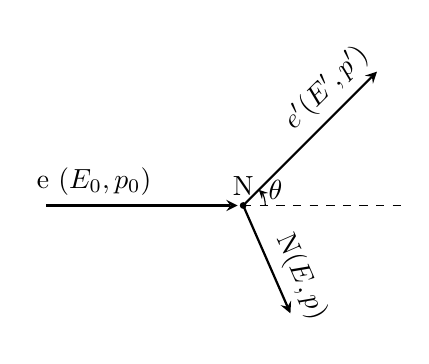
\begin{tikzpicture}
    \coordinate (N) at (0, 0);
    \coordinate (ein) at (-2.5, 0);
    \coordinate (eout) at (1.7, 1.7);
    \coordinate (p) at (0.6, -1.37);

    \filldraw[black] (N) circle (1pt);
    \node [above] at (N) {N};
    \draw[-stealth, thick] (ein) -- node [near start, above] {e ($E_0, p_0$)} ([xshift=-2pt]N);
    \draw[dashed] (N.east) -- +(2, 0);
    \draw[-stealth, thick] (N) -- node[near end, above, sloped] {$e' (E', p')$} (eout);
    \draw[-stealth, thick] (N) -- node[near end, above, sloped] {N($E, p$)} (p);
    \draw [-stealth] ([xshift=8pt]N) arc (0:45:8pt) node[right] {$\theta$};
\end{tikzpicture}
\end{center}

4-Momentum conservation 
$$ E_0 + M = E' + E \qquad \vec{p}_0 = \vec{p}' + \vec{p} $$
Assume ($m_e << 0 \Rightarrow E_0 \approx p_0, E' \approx p'$)
\begin{equation*}
    \begin{aligned}
	E^2 &= M^2 + \vec{p}^2 = M^2 + (\vec{p}_0 - \vec{p}')^2  \\
	    &= M^2 + (E_0 - E'\cos\theta)^2 + (E'\sin\theta)^2	\\
	    &= M^2 + E_0^2 + E'^2 - 2E_0E'\cos\theta	\\
	    &= (E_0 + M - E')^2
    \end{aligned}
\end{equation*}
So we can get
$$ M(E_0 - E') = E_0E'(1-\cos\theta) $$
$$ E' = \frac{ME_0}{M + E_0(1-\cos\theta)}$$
\begin{equation*}
    \begin{aligned}
	Q^2 &= -q^2 = -[(E_0 - E')^2 - (\vec{p}_0 - \vec{p}')^2]    \\
	    &= 2E_0E'(1-\cos\theta)
    \end{aligned}
\end{equation*}

%%%%%%%%%%%%%%%%%%%%%%%%
\section{Why Pb and Ca}
\begin{figure}
    \centering
    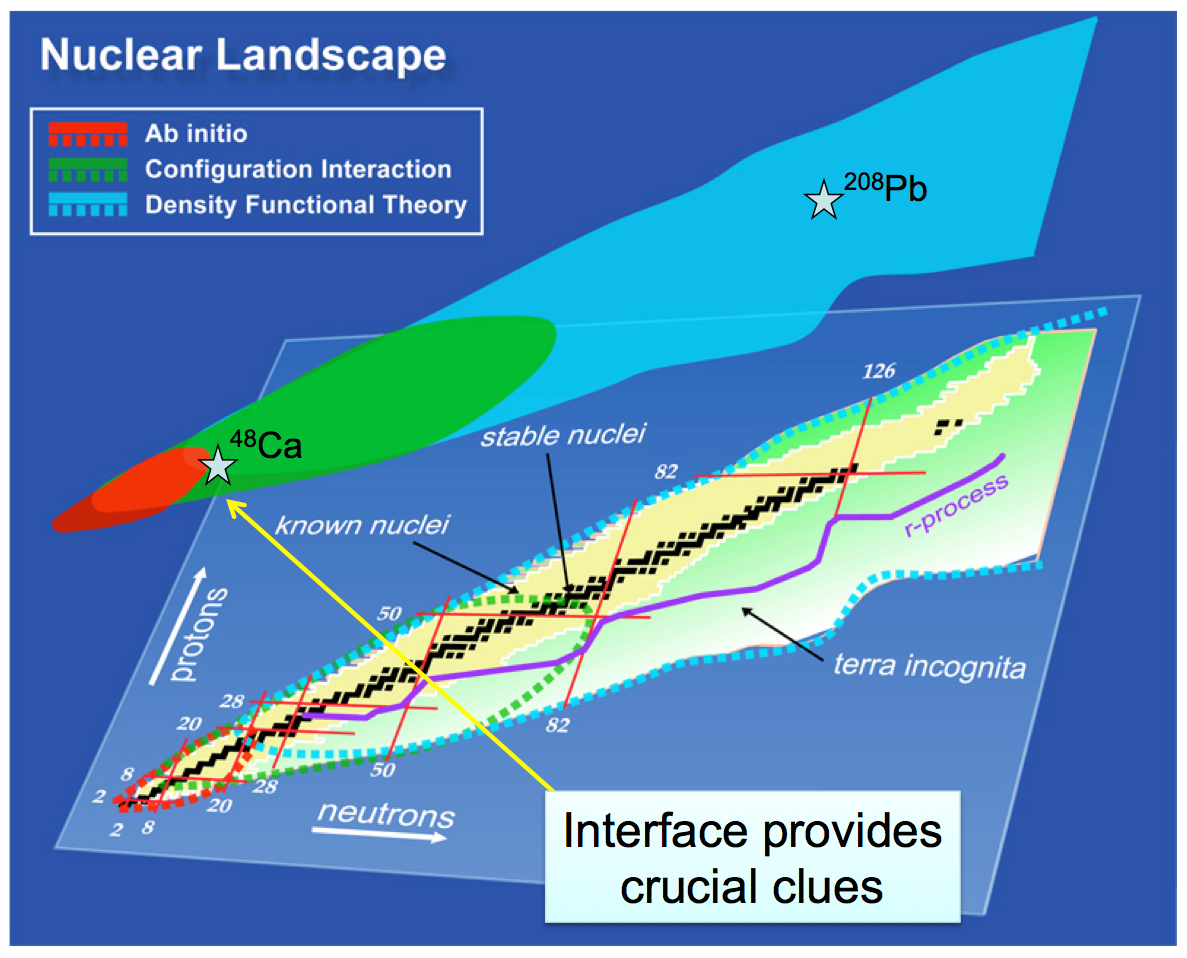
\includegraphics[width=0.6\linewidth]{Nuclear_Landscape}
    \caption{Nuclear Landscape}
    \label{fig:nuclear_landscape}
\end{figure}
As tiny as the neutron skin thickness, to measure it relatively accurate, the
larger it is, the better our measurement will be. So the target elements should
have a large neutron excess. So \Pb (\Ca) is chosed for PREX-II (CREX). Besides,
both nuclei are spin-0, so that we don't need to worry about the target 
polarization.
% what is the magic number: when a shell is completely filled, and the next higher
% energy shell is empty, the nucleus is said to have a magic number of proton 
% or neutrons
When the single nucleon seperation energy in a nucleus is much larger than that of
its neighbors, it is said that this nucleus has a magic number of protons or
neutrons. The magic number arises from the nucleon shell structure -- when 
a shell is fully filled and the next higher energy shell is empty, it is hard
to seperate out a nucleon from that closed shell.
Both \Ca and \Pb are doubly magic nuclei, which means both the number of protons
and neutrons are magic number, therefore a simple structure. 
It also means that the energy of their first 
excited state is much larger than the ground state, being 3.84 and 2.6 $MeV$ 
respectively. Combined with the high momentum resolution of HRS, it provides
sounding ground for flux integration detection.

As we see in previous section, the elastic scattering is quasi, not exact. The
small energy change is caused by nuclei recoil. The heavier the target nuclei,
the smaller the recoil effect, the smaller the $Q^2$, the better our measurement
of $Q^2$ and scattering angle.

Finally, \Ca, which lies in the medium region of the nuclear landscape, is 
accessible from both ab-initio and DFT theoretical approaches. 
By measuring the neutron skin thickness of \Ca, we hope to 
provides a possibility to bridge these two methods. 
